Ce chapitre décrit les différents diagrammes d'intéraction.

\section{Fonctionnalité 1}
Ce paragraphe décrit les diagrammes d'intéraction concernant la fonctionnalité 1. \\

La figure suivant (figure \ref{diagrammeInteraction1}) indique le déroulement de la création, la modification et la suppression d'un bénévole par un administrateur.
\begin{figure}[H]
	\centering
	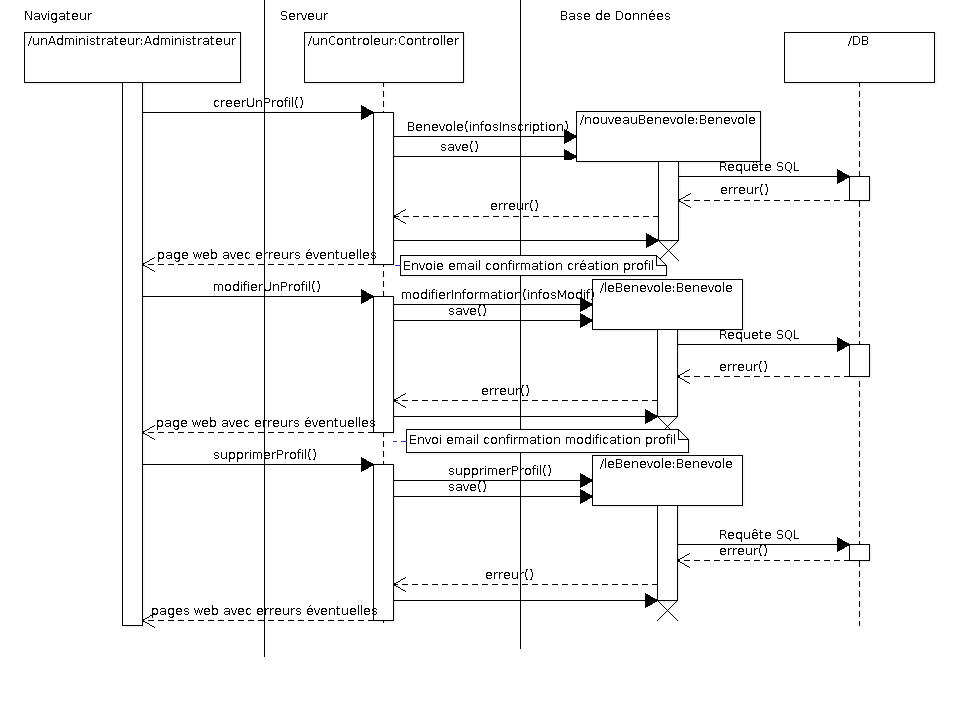
\includegraphics[scale=0.57]{images/diagrammesInteraction/01_diagrammeInteractionF1.png}
	\caption{Diagramme d'intéraction~: Création, modification, suppression d'un bénévole par un administrateur}
	\label{diagrammeInteraction1}
\end{figure}

La figure suivante (figure \ref{diagrammeInteraciton2}) indique le déroulement de la connexion et la déconnexion d'un bénévole.
\begin{figure}[H]
	\centering
	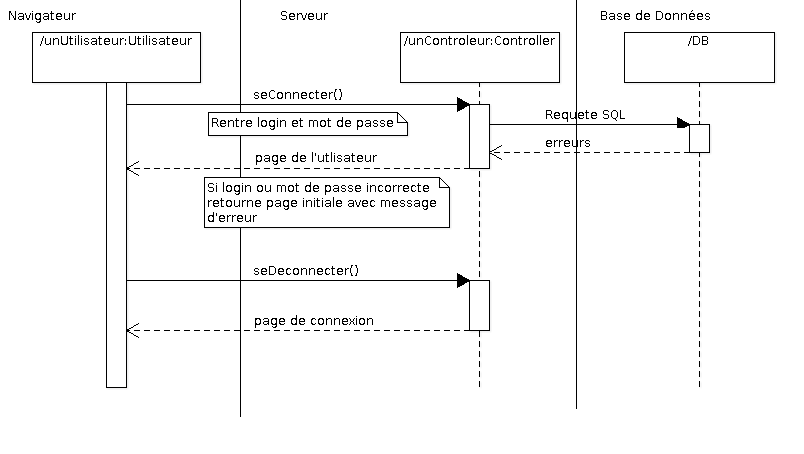
\includegraphics[scale=0.65]{images/diagrammesInteraction/02_diagrammeInteractionF1.png}
	\caption{Diagramme d'intéraction~: Connection et déconnection d'un utilisateur}
	\label{diagrammeInteraciton2}
\end{figure}

\section{Fonctionnalité 2}
Ce paragraphe décrit le diagramme d'intéraction concernant la fonctionnalité 2. \\

La figure suivante (figure \ref{diagrammeInteraction3}) indique le déroulement de la création, la modification et la suppression d'un établissement par un administrateur.
\begin{figure}[H]
	\centering
	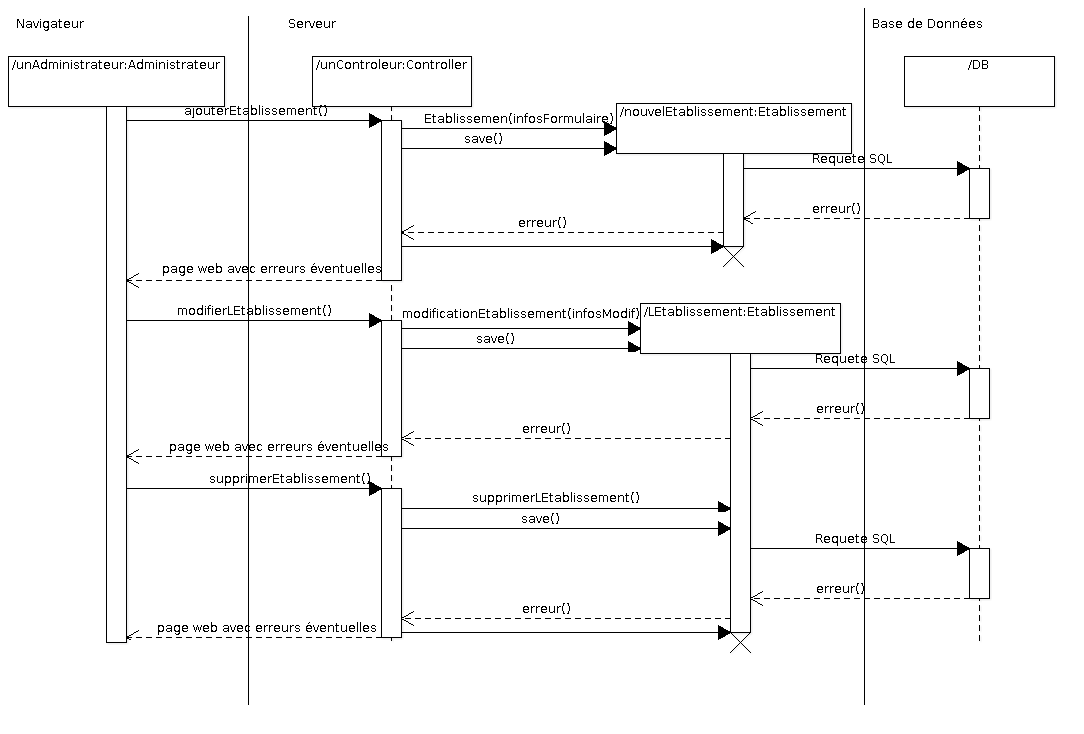
\includegraphics[scale=0.5]{images/diagrammesInteraction/03_diagrammeInteractionF2.png}
	\caption{Diagramme d'intéraction~: Création, modification, suppression d'un établissement par un administrateur}
	\label{diagrammeInteraction3}
\end{figure}

\section{Fonctionnalité 3}
Ce paragraphe décrit le diagramme d'intéraction concernant la fonctionnalité 3. \\

La figure suivante (figure \ref{diagrammeInteraction4}) indique le déroulement de l'envoi du formulaire de demande d'intervention aux établissements.
\begin{figure}[H]
	\centering
	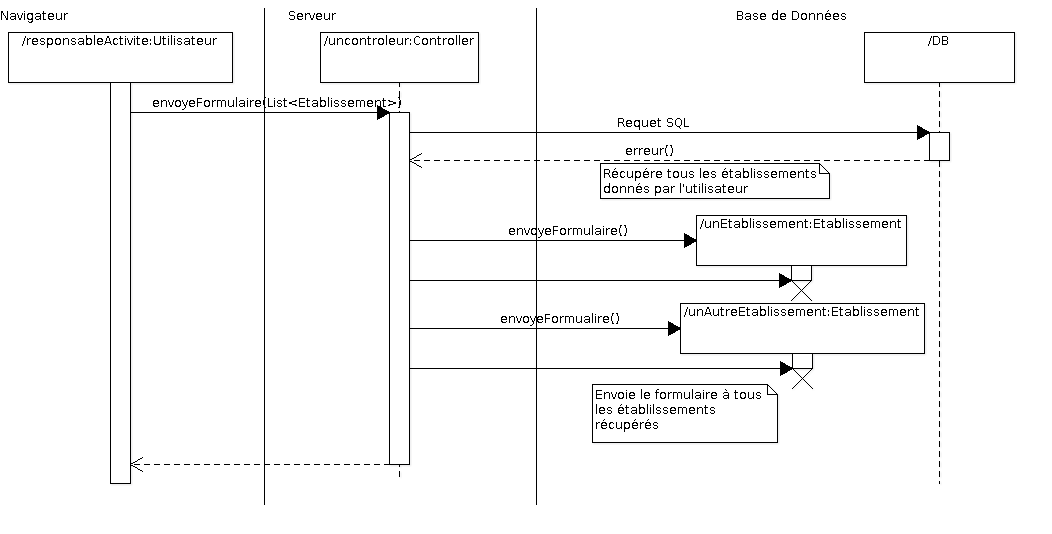
\includegraphics[scale=0.5]{images/diagrammesInteraction/04_diagrammeInteractionF3.png}
	\caption{Diagramme d'intéraction~: Envoye du formulaire à un ensemble d'établissement}
	\label{diagrammeInteraction4}
\end{figure}

\section{Fonctionnalité 4}
Ce paragraphe décrit les diagramme d'intéraction concernant la fonctionnalité 4. \\

La figure suivante (figure \ref{diagrammeInteraction5}) indique le déroulement du remplissage du formualaire de demande d'intervention.
\begin{figure}[H]
	\centering
	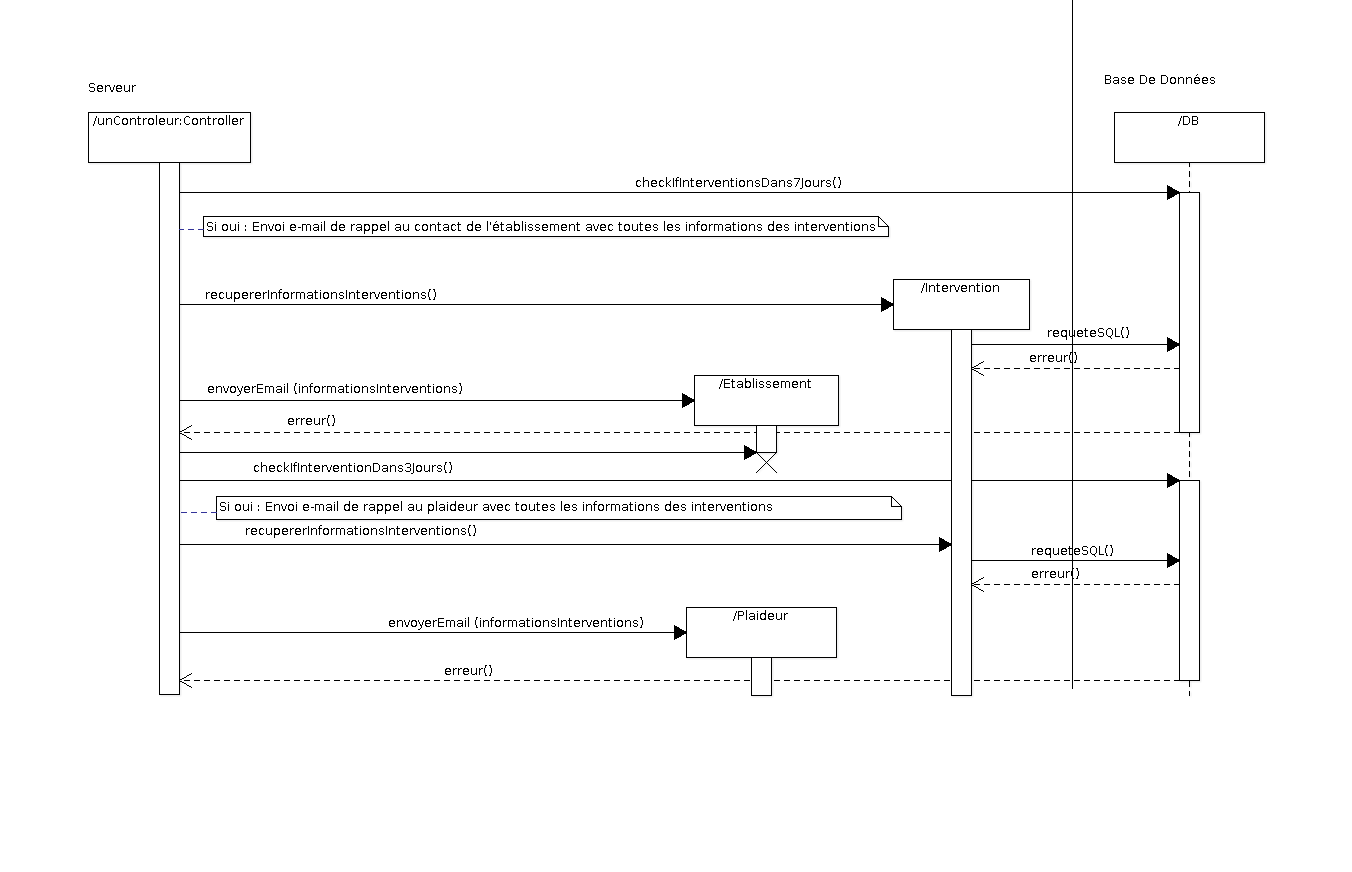
\includegraphics[scale=0.5]{images/diagrammesInteraction/05_diagrammeInteractionF4.png}
	\caption{Diagramme d'intéraction~: Replissage du formulaire}
	\label{diagrammeInteraction5}
\end{figure}


La figure suivante (figure \ref{diagrammeInteraction6}) indique le déroulement de l'annulation d'une demande d'intervention.
\begin{figure}[h]
	\centering
	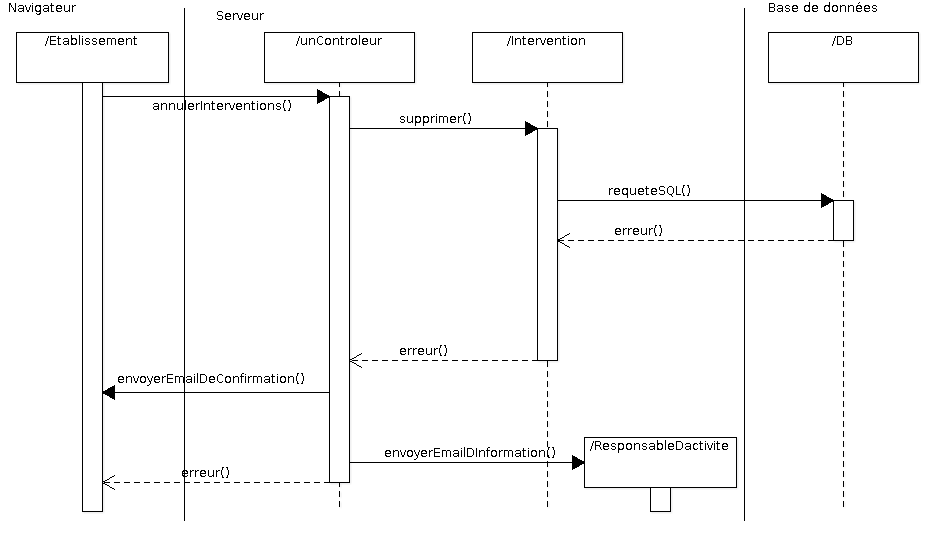
\includegraphics[scale=0.5]{images/diagrammesInteraction/06_diagrammeInteractionF4.png}
	\caption{Diagramme d'intéraction~: Annulation d'une demande d'intervention}
	\label{diagrammeInteraction6}
\end{figure}

\section{Fonctionnalité 5}
Ce paragraphe décrit le diagramme d'intéraction concernant la fonctionnalité 5. \\

La figure suivante (figure \ref{diagrammeInteraction7}) indique le déroulement de la géolocalisation des interventions ainsi que l'affectation d'un plaideur à celles ci. \\
\begin{figure}[H]
	\centering
	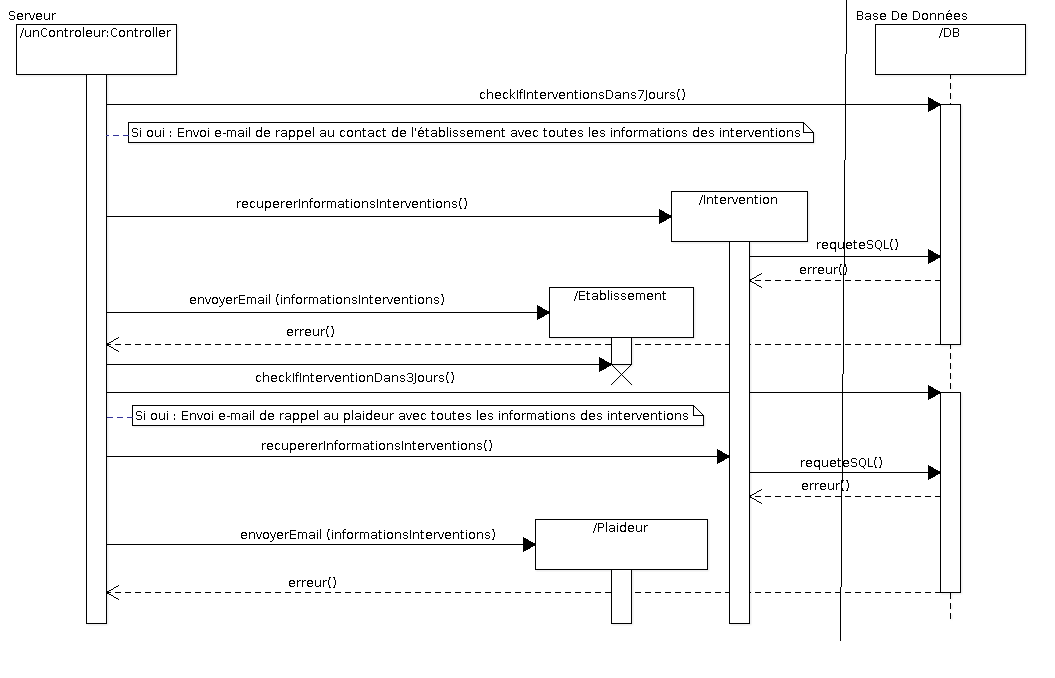
\includegraphics[scale=0.5]{images/diagrammesInteraction/07_diagrammeInteractionF5.png}
	\caption{Diagramme d'intération~: Géolocalisation des interventions et affectation à une intervention}
	\label{diagrammeInteraction7}
\end{figure}

\section{Fonctionnalité 6}
Ce paragraphe décrit le diagramme d'intéraction concernant la fonctionnalité 6. \\

La figure suivante (figure \ref{diagrammeInteraction8}) indique le déroulement de la mise à jour du planning d'un plaideur et l'information de prise en charge de l'intervention à l'établissement.
\begin{figure}[H]
	\centering
	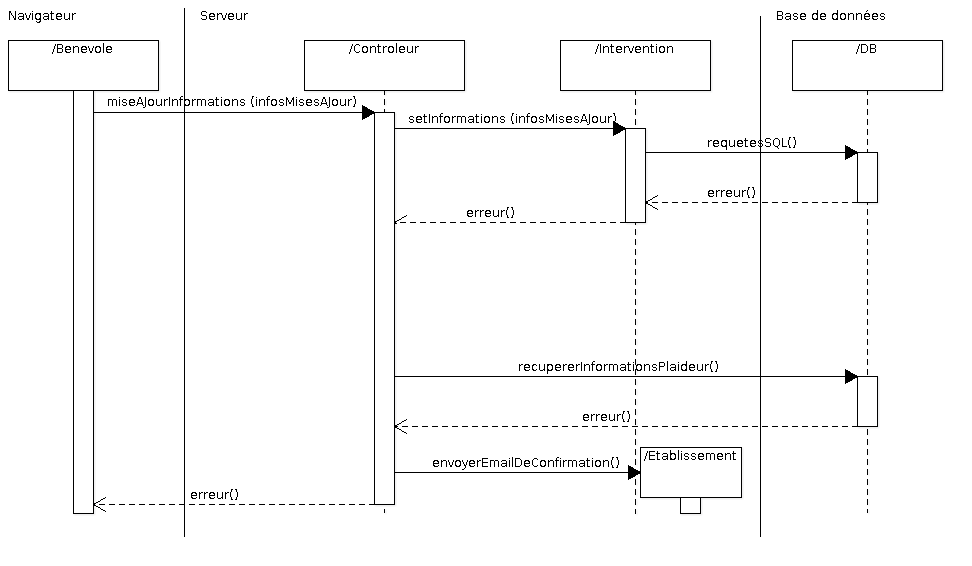
\includegraphics[scale=0.5]{images/diagrammesInteraction/08_diagrammeInteractionF6.png}
	\caption{Diagramme d'intéraction~: Mise à jour du planning d'un plaideur et information à l'établissement}
	\label{diagrammeInteraction8}
\end{figure}




\section{Fonctionnalité 7}
Ce paragraphe décrit le diagramme d'intéraction concernant la fonctionnalité 7.\\

La figure suivante (figure \ref{diagrammeInteraction9}) indique le déroulement de l'envoi des emails de rappel au plaideur et à l'établissement.
\begin{figure}[H]
	\centering
	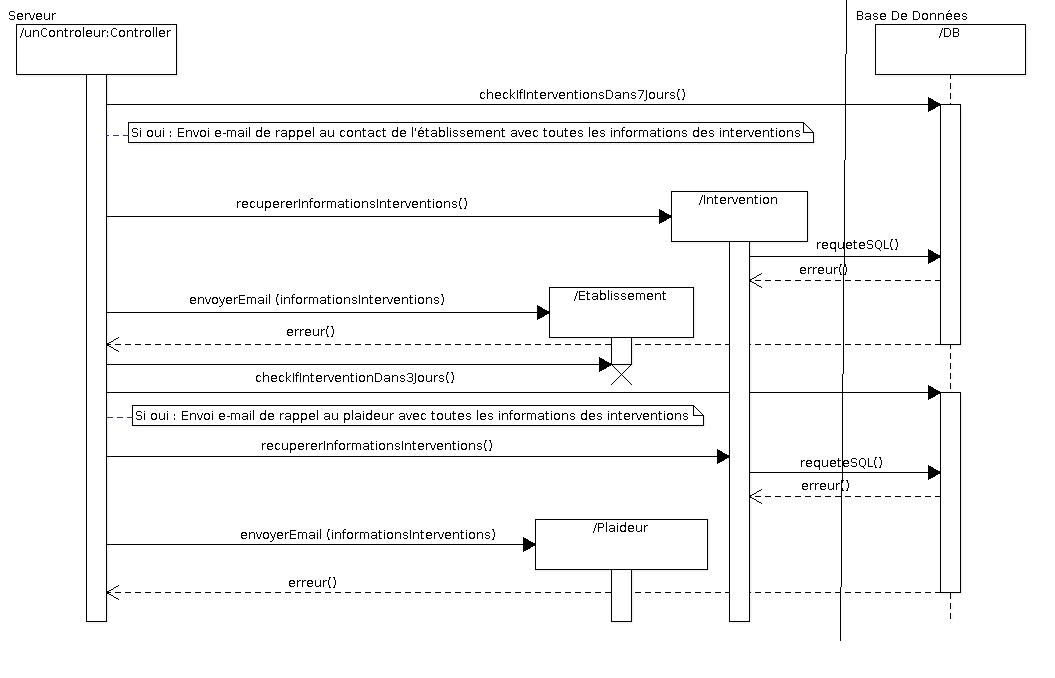
\includegraphics[scale=0.5]{images/diagrammesInteraction/09_diagrammeInteractionF7.png}
	\caption{Diagramme intéraction~: Envoi des emails de rappel}
	\label{diagrammeInteraction9}
\end{figure}